\subsubsection*{Module View}

This section provides us with three levels of abstractions of important set of functionalities that make up the system.
\vspace{3mm}

\underline{1. High Level Module View}
\vspace{3mm}

The view provides us with the high-level functionality of the project. Connections by arrows display dependent relationships between abstract packages.

\begin{figure}[h!]
    \centering
    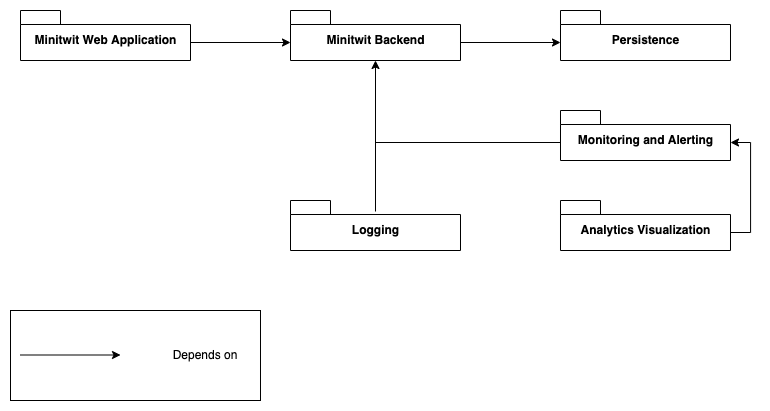
\includegraphics[width=\linewidth,height=\textheight,keepaspectratio]{images/architectural_views/minitwit_module_view_high_level.png}
    \caption{High level module view ~\cite{moduleViewHighLevel}}
    \label{fig:moduleview}
\end{figure}

\newpage

\underline{2. Layers of backend application}
\vspace{3mm}

This zoomed-in view with the architecture of the backend application shows the layering consisting of the Api, Domain Service and Persistence Layer.

\begin{figure}[h!]
    \centering
    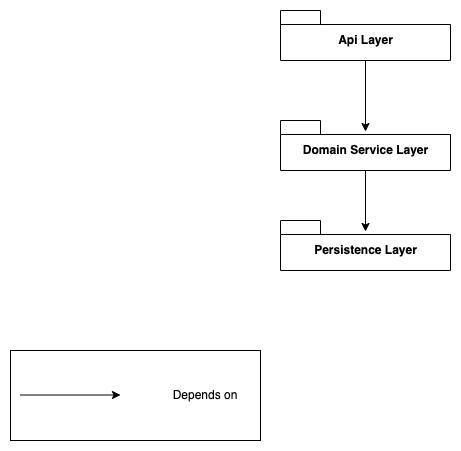
\includegraphics[width=0.5\textwidth]{images/architectural_views/minitwit_module_view_backend_layers.png}
    \caption{Layers of back-end ~\cite{moduleViewLayers}}
    \label{fig:modulebackend}
\end{figure}

\newpage
\underline{3. Layers detailed}
\vspace{3mm}

Focusing more into the architecture of the backend reveals a more in-depth structure of the layers. Controllers are dependent on DomainService classes that has access to Models representing data incoming from the Persistence Layer.

\begin{figure}[h!]
    \centering
    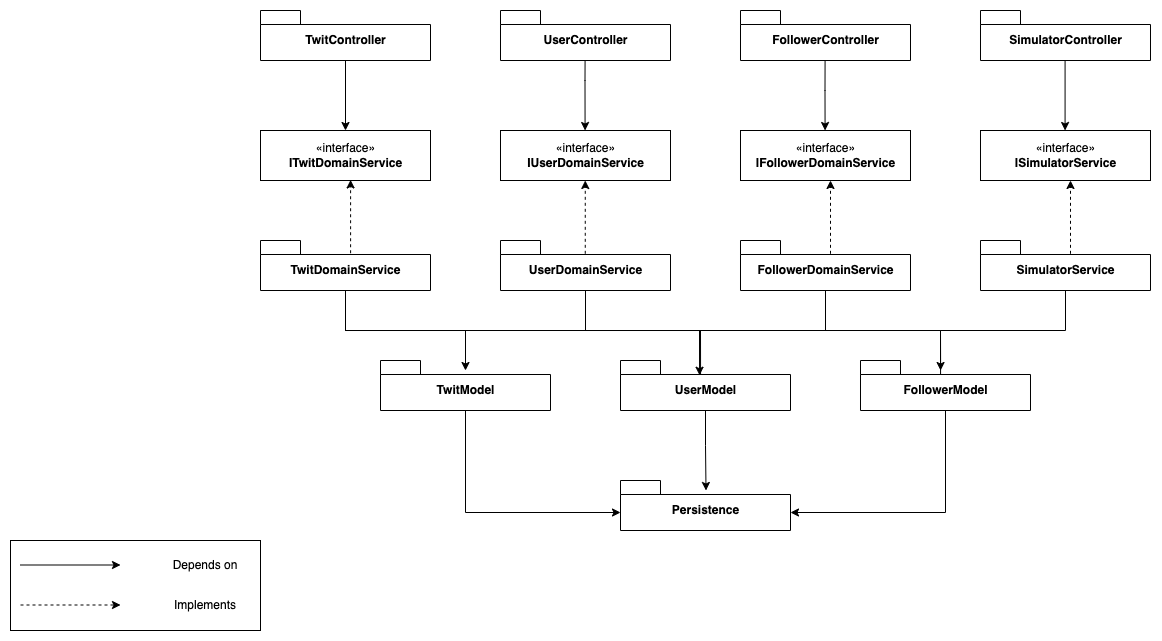
\includegraphics[width=\linewidth,height=\textheight,keepaspectratio]{images/architectural_views/minitwit_module_view_backend_layers_detailed.png}
    \caption{Layers detailed ~\cite{moduleViewLayersDetailed}}
    \label{fig:modulebackenddetail}
\end{figure}